\section{Practical Gradient Boosted Regression}
%
\begin{frame}[fragile]
Scikit-learn includes the gradient boosted regression algorithm in the \texttt{ensembles} module\\~\\

\begin{lstlisting}[language=python]
from sklearn.ensemble import GradientBoostedRegressor
\end{lstlisting}

\end{frame}
%
\begin{frame}[fragile]
A \texttt{GradientBoostingRegressor} object is fit in the same way as every other leaning model in sklearn\\~\\

\begin{lstlisting}[language=python]
model = GradientBoostingRegressor()
model.fit(X, y)
\end{lstlisting}

\end{frame}
%
\begin{frame}[fragile]
The \texttt{predict} method returns predictions on new data\\~\\

\begin{lstlisting}[language=python]
preds = model.predict(X_new)
\end{lstlisting}

Especially useful is the iterator \texttt{staged\_predict} which creates predictions from models created by truncating series of trees\\~\\

\begin{lstlisting}[language=python]
for preds in model.staged_predict(X_new):
    # Do something interesting, used heavily in the plots to follow.
\end{lstlisting}

\end{frame}
%
\begin{frame}[fragile]

\texttt{GradientBoostingRegressor} has many knobs to turn.\\~\\

\begin{lstlisting}[language=python]
GradientBoostingRegressor(loss='ls',
                          n_estimators=100, 
                          learning_rate=0.1,
                          max_depth=3,
                          subsample=1.0, 
                          min_samples_split=2, 
                          min_samples_leaf=1, 
                          min_weight_fraction_leaf=0.0,
                          ...)
\end{lstlisting}

\end{frame}
%
\begin{frame}[fragile]
The most important options to \texttt{GradientBoostedRegressor} are

\begin{itemize}
  \item \texttt{loss} controls the loss function to minimize.  \texttt{ls} is the least squares minimization algorithm we discussed in the previous section.
  \item \texttt{n\_estiamtors} is how many boosting stages to compute, i.e. how many regression trees to grow.
  \item \texttt{learning\_rate} is the learning rate for the gradient update.
  \item \texttt{max\_depth} controls how deep to grow each individual tree.
  \item \texttt{subsample} allows to fit each tree on a random sample of the training data (like bagging in random forests).
\end{itemize}

\end{frame}
%
\begin{frame}{Tuning the Number of Estimators}

As more and more trees are added to the model the training set error will be driven down monotonically, but the same is not true for the testing error

  \begin{figure}
    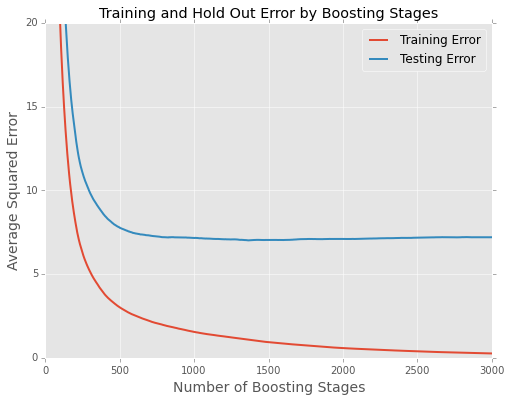
\includegraphics[scale=0.45]{training-and-testing-error}
  \end{figure}

\end{frame}
%
\begin{frame}

  \begin{figure}
    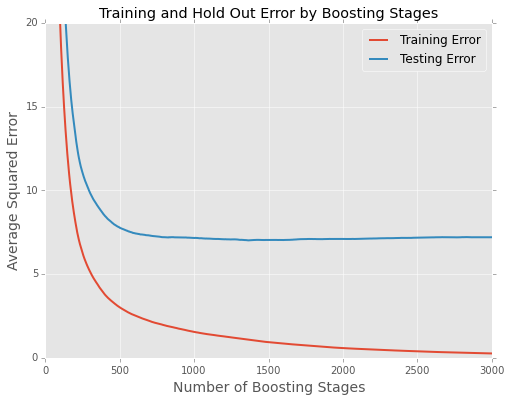
\includegraphics[scale=0.45]{training-and-testing-error}
  \end{figure}

This means that it is essential to determine the proper number of trees to grow, as too many may lead to overfitting

\end{frame}
%
\begin{frame}
One way to tune the numer of trees is to make use of a validation set, held out from both training and testing

  \begin{figure}
    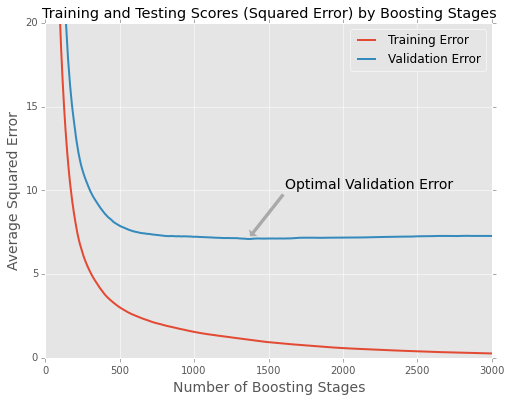
\includegraphics[scale=0.45]{training-and-testing-error-with-optima}
  \end{figure}
  
\end{frame}
%
\begin{frame}[fragile]
The \texttt{loss\_} method is important here, it allows us to compute the loss function on held out data\\~\\

\begin{lstlisting}[language=python]
def get_optimal_n_estimators(model, X_new, y_new):
    validation_loss = np.zeros(
        model.get_params('n_estimators'))
    for i, preds in enumerate(model.staged_predict(X_new)):
        validation_loss[i] = model.loss_(preds, y_new)    
    optimal_tree = np.argmin(validation_loss)
    optimal_loss = validation_loss[optimal_tree]
    return optimal_tree, optimal_loss
\end{lstlisting}

\end{frame}
%
\begin{frame}[fragile]
One the optimal number of estimators is known, it's useful to truncate the model\\~\\

\begin{lstlisting}[language=python]
from copy import deepcopy

def truncate_boosted_model(model, n_estimators):
    new_model = deepcopy(model)
    # Two dimensions here for the case of multiple classes
    # in a GradientBoostedClassifier.
    new_model.estimators_ = model.estimators_[:n_estimators, :]
    new_model.n_estimators = n_estimators
    return new_model
\end{lstlisting}

\end{frame}
%
\begin{frame}
Another way to choose the optimal number of trees is to replace the validation set with cross validation

  \begin{figure}
    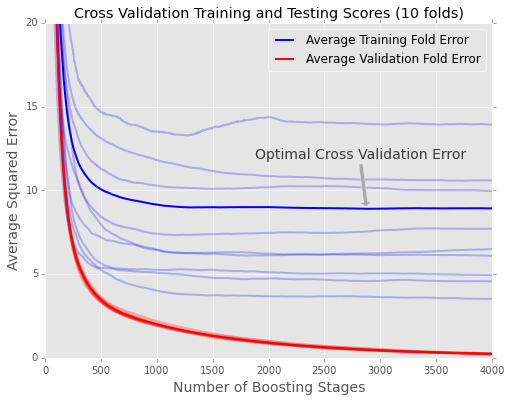
\includegraphics[scale=0.45]{training-and-testing-cv-error}
  \end{figure}
  
\end{frame}
%
\begin{frame}

  \begin{figure}
    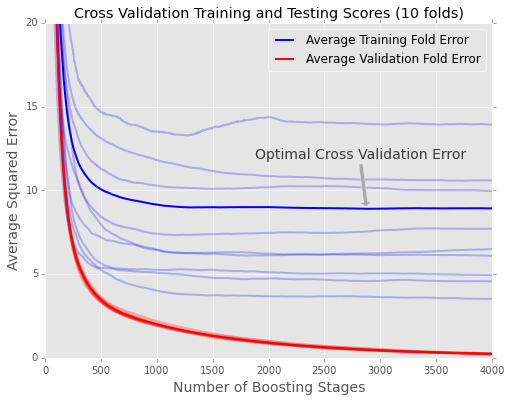
\includegraphics[scale=0.45]{training-and-testing-cv-error}
  \end{figure}
  
We generally choose the number of trees minimizing the \textit{average} out validation fold error.

\end{frame}
%
\begin{frame}{Tuning the Learning Rate}

The learning rate allows us to grow our boosted model slowly.\\~\\

A large learning rate will cause the model to fit hard to the training data, which creates a \textit{high variance} situation.\\~\\

A smaller learning rate reduces the boosted models sensitivity to the training data.\\~\\

\end{frame}
%
\begin{frame}
Decreasing the learning rate reduces how fast the booster drives down the training error rate
  \begin{figure}
    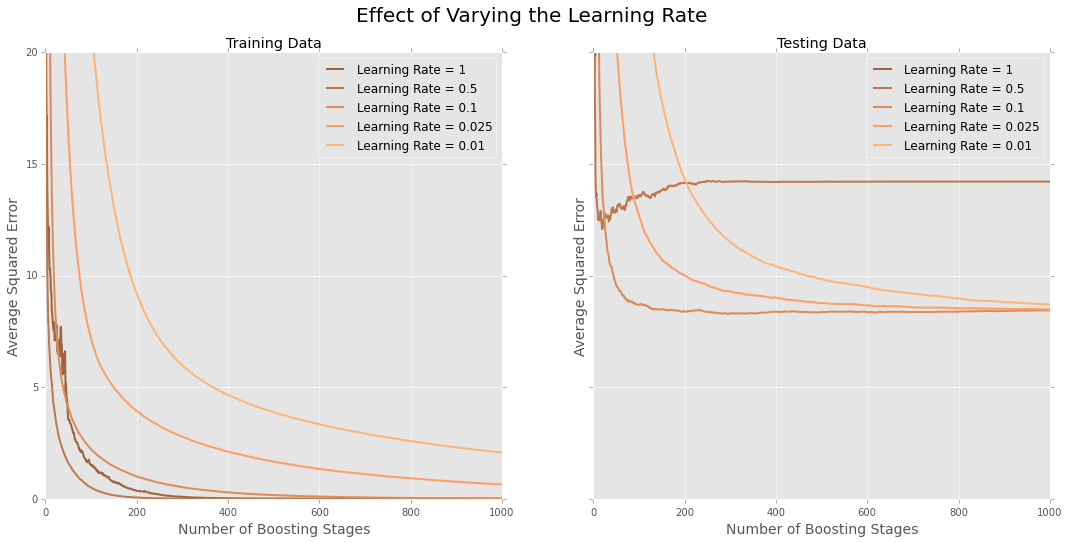
\includegraphics[scale=0.30]{varying-learning-rate-error}
  \end{figure}
  
\end{frame}
%
\begin{frame}
On the other hand, a smaller learning rate means more trees are needed to reach the optimal point

  \begin{figure}
    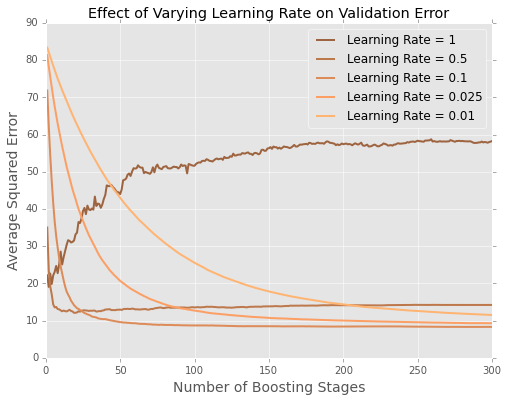
\includegraphics[scale=0.50]{varying-learning-rate-error-testing-zoom-start}
  \end{figure}
  
\end{frame}
%
\begin{frame}
In general, a smaller learning rate eventually (over enough time) results in a superior model

  \begin{figure}
    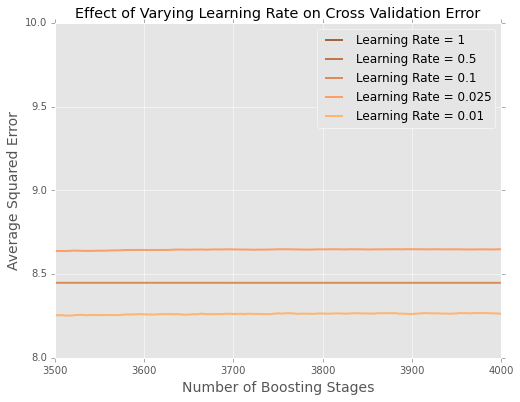
\includegraphics[scale=0.50]{varying-learning-rate-error-testing-zoom-end}
  \end{figure}
  
\end{frame}
%
\begin{frame}
\textbf{Strategy for Learning Rate}:

\begin{itemize}
  \item In the initial exploratory phases of modeling, set the learning rate to some large value, say $0.1$.  This allows you to iterate through ideas quickly.
  \item When tuning other parameters using grid search, decrease the learning rate to a more sensible value, $0.01$ works well.
  \item When fitting the \textit{final} production model, set the learning rate to a very small value, $0.001$ or $0.0005$, smaller is better.
\end{itemize}

\end{frame}
%
\begin{frame}
\textbf{General Advice:}\\~\\

Run the final model overnight!  It will fit while you are sleeping!\\~\\

Make sure you've written all your analysis code up front, based on your initial models.  Then all that's left is to run your final model through and see your final plots and statistics.
\end{frame}

%
\begin{frame}{Tuning the Tree Depth}
A larger tree depth allows the model to capture deeper interactions between the predictors, resulting in lower bias.

  \begin{figure}
    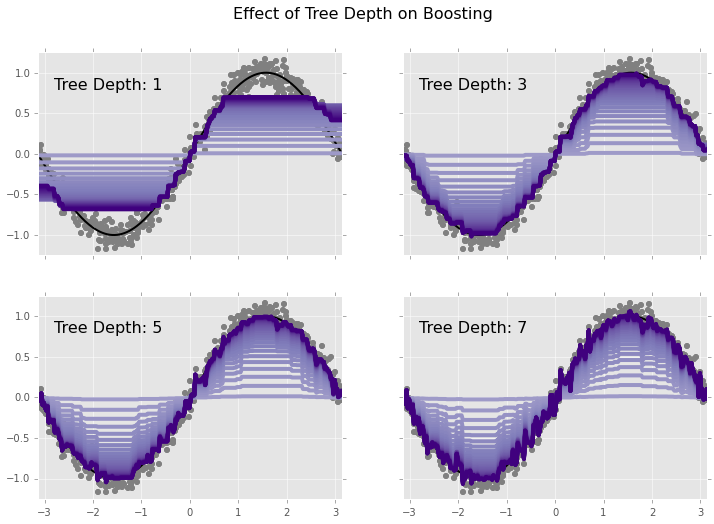
\includegraphics[scale=0.3]{sin-changing-depth}
  \end{figure}

\end{frame}
%
\begin{frame}
A deeper tree depth also

\begin{itemize}
  \item Causes the model to fit faster, increasing the variance and somewhat combating the effect of the learning rate.
  \item Allows the model to assume a more complex for at the same number of trees.  This is a blessing (low bias) and curse (high variance).
\end{itemize}
\end{frame}
%
\begin{frame}
It's never obvious up front what tree depth is best for a given problem, so a grid search is needed to determine the best value

  \begin{figure}
    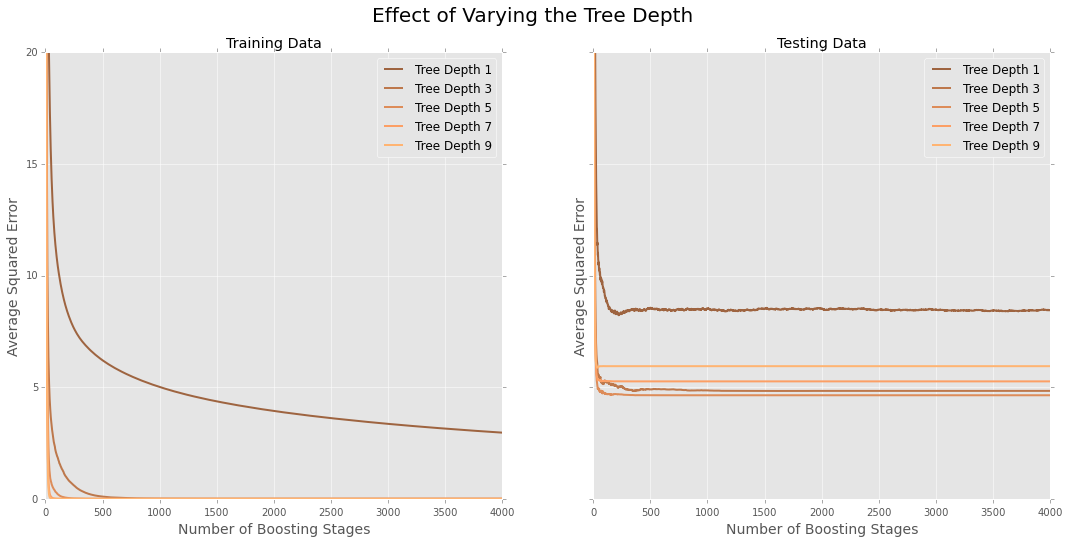
\includegraphics[scale=0.50]{varying-tree-depth-error}
  \end{figure}
  
\end{frame}
%
\begin{frame}

  \begin{figure}
    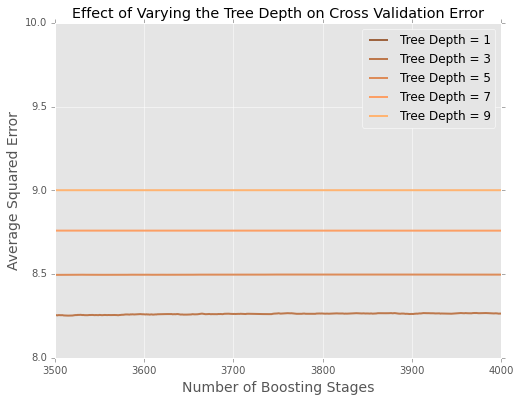
\includegraphics[scale=0.50]{varying-tree-depth-error-zoom}
  \end{figure}
  
\end{frame}
%
\begin{frame}
\textbf{Strategy for Tree Depth}:

Tune with a grid search and cross validation.
  
\end{frame}
%
\begin{frame}{Tuning the Subsample Rate}
The \texttt{subsample} parameter allows one to train each tree on a subsample of the training data.\\~\\

This is similar to bagging in the random forest algorithm, and has the same result: it lowers the variance of the resulting model.
\end{frame}
%
\begin{frame}
Not subsampling at all, or over subsampling are both bad ideas

  \begin{figure}
    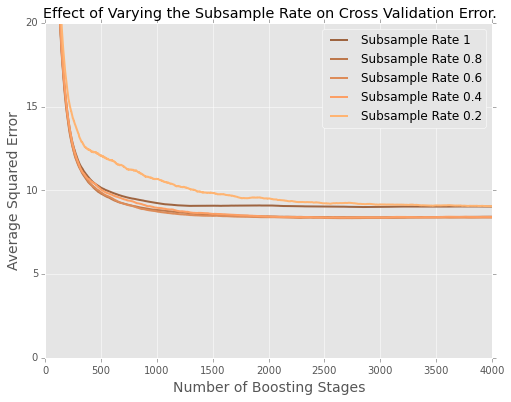
\includegraphics[scale=0.50]{varying-subsample-rate-error}
  \end{figure}
 
\end{frame}
%
\begin{frame}
Between these two extremes, different levels of subsampling generally give the same performance

  \begin{figure}
    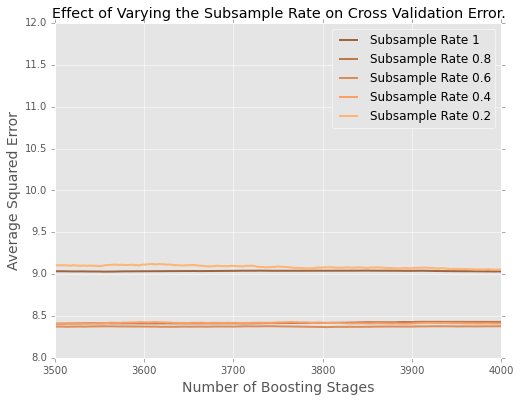
\includegraphics[scale=0.50]{varying-subsample-rate-error-zoom-end}
  \end{figure}
  
\end{frame}
%
\begin{frame}
\textbf{Strategy For Subsample:}\\~\\

Set to $0.5$, it almost always works well.\\~\\

If you have a massive amount of data and want the model to fit more quickly, decrease this value.
\end{frame}
%
\begin{frame}{Tuning Other Gradient Boosting Parameters}

The other parameters to \texttt{GradientBoostingRegressor} are less important, but can be tuned with grid search for additional improvements in importance.

\begin{itemize}
  \item \texttt{min\_samples\_split}: Any node with less samples than this will not be considered for splitting.
  \item \texttt{min\_samples\_leaf}: All terminal nodes must contain more samples than this.
  \item \texttt{min\_weight\_fraction\_leaf}: Same as above, but a expressed as a fraction of the total number of training samples.
\end{itemize}

\end{frame}
%
\begin{frame}
Generally these are less important because \textit{you shouldn't be growing super gigantic trees}!\\~\\

\only<2->{
If you \textit{do} decide to include these in a grid search, \textit{be wary of overfitting to your validation set}.\\~\\
}

\only<3->{
\textit{The number of model comaprisons grows exponentially in the number of parameters tuned.}
}
\end{frame}
%
\begin{frame}{Max Features}
There's one more parameter worth mentioning\\~\\

\texttt{max\_features}: The number of features to consider for each split, as in random forest.\\~\\

\textbf{Exercise}: Think about how varying this parameter will influence the model.  Run some experiments to see if you're right.  Should you include this in a grid search?
\end{frame}
  
  